\documentclass[12pt]{article}
\usepackage[utf8]{inputenc}
%\usepackage[latin1]{inputenc}
\usepackage[T1]{fontenc}
\usepackage[english]{babel}
\usepackage{graphicx}
\usepackage{amsmath}
\usepackage{amsfonts}
\usepackage{amssymb}
\usepackage{fancyhdr}
%\usepackage[nottoc, notlof, notlot]{tocbibind}
\usepackage{geometry}
%\geometry{ hmargin=3.2cm, vmargin=4cm }
%\usepackage{graphicx}
\usepackage{hyperref}

\DeclareMathOperator*{\Max}{Max}
\DeclareMathOperator*{\Argmax}{Argmax}
\newcommand{\E}[1]{\mathbb{E}_{#1}}
\newcommand{\dpp}[2]{\frac{\partial #1}{\partial #2}}
\newcommand{\ddpp}[2]{\frac{d #1}{d #2}}
\newcommand{\ti}[1]{\widetilde{#1}}
\newcommand{\ub}[2]{\underbrace{#1}_{#2}}
\newcommand{\ubt}[2]{\underbrace{#1}_{\text{#2}}}
\newcommand{\oomega}[0]{\overline{\omega}}
\newtheorem{lemma}{Lemma}
\newtheorem{definition}{Definition}
\newtheorem{proposition}{Proposition}
\newtheorem{assumption}{Assumption}

\setlength{\parindent}{20pt}
\setlength{\parskip}{1ex plus 4.ex minus .2ex}
%\linespread{1.2}



\title{Best Ideas, Idiosyncratic Shocks and Aggregate Fluctuations}

\author{Basile Grassi\\
\small{\emph{Paris School of Economics and Université Paris 1 Panthéon Sorbonne}}
}

\date{\today}

\begin{document}
\maketitle

\begin{abstract}
This paper derives a model of aggregate fluctuations from idiosyncratic shocks. An endogeneous fat-tailed distribution of firms size arises because of selection of the best ideas \emph{\`a la} Alvarez \emph{et al.} (2008) \nocite{Alva08}. An entrepreneur update its idea only if it improves its technology. This leads to growth and a fat-tailed distribution of firms sizes. From this, idiosyncratic shocks leads to aggregate fluctuations as in Gabaix (2011) \nocite{Gaba11}.
\end{abstract}



\section{Selection of ideas}

Following Alvarez \emph{et al.} (2008) \nocite{Alva08} and Lucas (2009)\nocite{Luca09}, the technology frontier evolves according to a differential equation. This differential equation depends on the way the flow of ideas is modeled.

Let us denote $X$ the cost level (the average TFP will be $1/X$) and $G(x,t)$ the counter cumulative distribution function, i.e.
\begin{equation*}
\mathbb{P}_t\{X \geq x\} = G(x,t)
\end{equation*}
We will call $X$ an idea or a cost level.

\subsection{Poisson arrivals with internal source of ideas}
An entrepreneur at $t$  inherits cost level and receives a new idea drawn from the current distribution $G(x,t)$ at a Poisson arrrival rate $\alpha$. She keeps the new idea only if it is a better idea that is to say that the new cost is lower the current one.

For fixed $x$, I follow Alvarez \emph{et al.} (2008) \nocite{Alva08} to motivate  an ordinary differential equation:

\begin{equation*}
G(x,t+h)=G(x,t)  \mathbb{P} \{ \text{no lower cost arrives in } (t,t+h) \} 
\end{equation*}

Then
\begin{align*}
\mathbb{P} \{ \text{no lower cost arrives in } (t,t+h) \} &=  \mathbb{P} \{ \text{no ideas arrives in } (t,t+h) \} \\
&+ \mathbb{P} \{ \text{one idea } > x \text{ arrives from } G \text{ in }  (t,t+h) \} \\
&+ \mathbb{P} \{ \text{more than on idea } > x \text{ arrives in } \text{ in }  (t,t+h) \} \\
&= 1 - \alpha h + \alpha h G(x,t) + o(h)
\end{align*}
which yields after some computations (rearranging and dividing through by $h$, and letting $ h \rightarrow 0$):
\begin{equation*}
\dpp{\log(G(x,t))}{t}= - \alpha [ 1-G(x,t) ] 
\end{equation*}

The solution of this equation is 
\begin{equation*}
G(x,t) = \frac{G(x,0)}{G(x,0)+ e^{\alpha t}(1-G(x,0))} 
\end{equation*}

We are a focusing on a ``balanced growth path'' which is to say whether there is a function $\varphi$ and a number $\nu$ such that
\begin{equation*}
G(x,t)=\varphi(e^{\nu t} x) 
\end{equation*}
which after choosing $\nu=\alpha$  and some computations leads to
\begin{equation*}
\varphi'(x)=-\frac{1}{x} \varphi(x)(1-\varphi(x))
\end{equation*}
which has a solution $\varphi : \mathbb{R}_+ \rightarrow [0,1]$
\begin{equation*}
\varphi(x)=\frac{1}{1+\phi x}  = \mathbb{P} \{ X \geq x\}
\end{equation*}
where $\phi$ is a parameter.

Alavarez \emph{et al.} (2008) shows that given an initial distribution $G(x,0)$, $\lim_{t\rightarrow 0} G(e^{-\alpha t}x,t) = \varphi (x)$ and that $\phi = -G_x(0,0)$.

Thus the distribution of cost $X$ is characterized by the counter cumulative distribution function (CCDF) $\varphi(.)$ and then the average TFP is defined by $Y=\tfrac{1}{X}$. The distribution of $Y$ is characterized by a CCDF 

\begin{align*}
\mathbb{P} (Y \geq y) = \mathbb{P} (\frac{1}{X}\geq y) &= \mathbb{P} (\frac{1}{y}\geq X) \\
&= 1 - \mathbb{P} ( X >  \frac{1}{y}) \\
&= 1 - \frac{1}{1+ \phi \frac{1}{y}} \\
&= \frac{\phi \frac{1}{y} }{1+ \phi \frac{1}{y}} \\
\mathbb{P} (Y \geq y) &= \frac{1}{1+ \frac{y}{\phi}} := g(y)
\end{align*}



%\subsection{Poisson arrivals with external source of ideas and growth in the arrival rate}

%Leads to an asymptotic exponential distribution with parameter $-\beta H'(0)$ of $G(x,t)$. 

\section{A simple model of aggregate fluctuations from idiosyncratic shocks}

\subsection{Environment}
This economy is populated by $N$ entrepreneurs who draw ideas $\varphi$ from the stationary distribution of ideas characterized by $g(.)$, they keep this ideas during the two periods of this economy.

They are endowned with a technology from which they produce $z n^{\alpha} $ units of final good with $n$ units of input at cost $w$ per unit of final output. The TFP term $z$ is at the first period $z_1=\varphi^{1-\alpha}$ and at the second period $z_2 = f(\varphi, x)^{1-\alpha}$ where $x$ is drawn from a given distribution characterized by a probability distribution $h(.)$\footnote{$x$ could be interpreted as the relative growth of its ideas compare to the balanced growth of each ideas. Here we suppose that the draw of $y$ and the draw of $x$ are independant.} and $f(.,.)$ will be defined later\footnote{The hypothesis that $z_1=\varphi^{1-\alpha}$ and $z_2 = f(\varphi, x)^{1-\alpha}$ is critical. Because this hypothesis leads to a one to one mapping between the tail parameter of the size distribution of firms and the one of the productivity distribution. Whitout this hypothesis the tail parameter will be $\frac{1}{1-\alpha} \approx 3$ which implies a thin tail distribution of firms size.}.

For a given productivity level $z$, each entrepreneur maximizes its profit. Thus the program of the entrepreneur is:
\begin{equation*}
\pi (z,w) = \max_{n\geq 0} \{ z n^{\alpha} - w n\} 
\end{equation*}
which leads to 
\begin{align*}
\text{Input demand:   }  n^*(z,w) &=  \Big( \frac{z \alpha}{w} \Big)^{\frac{1}{1-\alpha}}  \\
\text{Supply of final good:   }y^*(z,w) &= z^{\frac{1}{1-\alpha}} \big( \frac{\alpha}{w} \big)^{\frac{\alpha}{1-\alpha}}\\
\text{Profit:   }\pi^*(z,w) &= z^{\frac{1}{1-\alpha}} \big( \frac{1}{w} \big)^{\frac{\alpha}{1-\alpha}} \alpha^{\frac{1}{1-\alpha}} (\frac{1}{\alpha}-1)\\
\end{align*}

For a given ideas $y$ and a given ability $x$ the output at the first period is $y_1 = \varphi \big( \frac{1}{w} \big)^{\frac{\alpha}{1-\alpha}} \alpha^{\frac{1}{1-\alpha}} (\frac{1}{\alpha}-1)$ and $y_2 = f(\varphi, x) \big( \frac{1}{w} \big)^{\frac{\alpha}{1-\alpha}} \alpha^{\frac{1}{1-\alpha}} (\frac{1}{\alpha}-1)$.

At this point, an entrepreneur $i\in \{1,2,\ldots, N\}$ is characterized by $(\varphi_i,x_i)$ where $\varphi_i$ stand for the idea and $x_i$ the idiosyncratic shock in the second period. She produces $y_1^i$ and $y_2^i$ in the first and the second period respectively.

\subsection{Aggregate volatility}

The total GDP of this economy is just the sum over the entrepreneurs of each production $y_t^i$:
\begin{equation*}
 Y_t = \sum_{i=1}^N y_t^i
\end{equation*}


The GDP growth is defined by
\begin{equation}
\label{GDP}
\frac{\Delta Y_{t+1}}{Y_t} = \frac{1}{Y_t} \sum_{i=1}^N  \Delta y^i_{t+1}
\end{equation}

The absolute growth of a firm own by the entrepreneur $i$ is 
\begin{equation*}
\Delta y^i_{t+1}=  \big( \frac{\alpha}{w} \big)^{\frac{\alpha}{1-\alpha}} \Big(  f(\varphi_i,x_i) -\varphi_i \Big)\\
\end{equation*}

Let us assume that $f(\varphi_i,x_i) = \varphi_i  x_i$ which yields\footnote{This assumption is also key, since for $f(\varphi_i,x_i) = \varphi_i + x_i$, $\Delta y^i_{t+1}$ will not be proportional to $y^i_{idea}$ and Gabaix' theorem does not applied anymore.}.
\begin{align*}
\Delta y^i_{t+1}&=  \Big( \frac{\alpha}{w} \Big)^{\frac{\alpha}{1-\alpha}} \varphi_i ( x_i - 1 )\\
 &= y^i_{idea} ( x_i - 1 )
\end{align*}
where $y^i_{idea} := \Big( \frac{\alpha}{w} \Big)^{\frac{\alpha}{1-\alpha}} \varphi_i$\footnote{Here $ y^i_{idea}= y^i_t$}. From this equation, one can see that the growth of firm follow a Gibrat's law - the growth of firm does not depend on its size\footnote{This will be false as soon as in the first period a ability shock is drawn by the entrepreneur. In this last case $\Delta y^i_{t+1} = y^i_{idea} ( x^i_{t+1} - x^i_t )$. in this last case all the following result are still true.}.

Finally, the GDP is thus
\begin{equation*}
\frac{\Delta Y_{t+1}}{Y_t} = \frac{1}{Y_t} \sum_{i=1}^N y^i_{idea} ( x_i - 1 )
\end{equation*}
from which, I can derive the GDP volatility
\begin{equation*}
  \sigma_{GDP} = \sqrt{\mathbb{V}ar_t \Big( \frac{\Delta Y_{t+1}}{Y_t} \Big) } = \Big( \sum_{i=1}^N \sigma^2 \Big( \frac{y^i_{idea}}{Y_t} \Big)^2 \Big)^{1/2}
\end{equation*}
where $\sigma^2$ is the variance of the idiosyncratic shock $h(.)$.

Let us compute the distribution from which $y^i_{idea}$ are drawn.
\begin{align*}
\mathbb{P}\{ y_{idea} > y \} &= \mathbb{P}\{ \Big( \frac{\alpha}{w} \Big)^{\frac{\alpha}{1-\alpha}} \varphi > y \} \\
&= \mathbb{P}\Big\{  \varphi > \frac{y}{( \frac{\alpha}{w} )^{\frac{\alpha}{1-\alpha}} } \Big\} \\
&= g\Big(\frac{y}{( \frac{\alpha}{w} )^{\frac{\alpha}{1-\alpha}} }\Big)\\
&=  \frac{1}{1+\frac{y}{\phi( \frac{\alpha}{w} )^{\frac{\alpha}{1-\alpha}} }}
\end{align*}
this distribution does not have a variance.

From this one can apply Proposition 2 from Gabaix (2011)  \nocite{Gaba11} and conclude that $\sigma_{GDP} \sim \frac{v}{\ln N}\sigma$, where $v$ is a random variable following a distribution which does not depend on $N$ or $\sigma$\footnote{$v$ follow the square root of a stable l\'evy distribution with exponent $1/2$.}.

\subsection{Simulation}

I assume that the idiosyncratic shock $x$ is equal to $\exp(s)$ where $s$ follow a normal distribution with mean 0 and variance $\sigma^2$. The parameters value are $\phi=2, \alpha=0.6, w=0.3$ and $\sigma=0.01$. To compute figure \ref{Emp_std}, for each number of firms $N$, I draw $M=1000$ economies. Each economy is characterized by a sequence $\{ (\varphi_i,x_i)\}_{1 \ldots N}$. For each economy, I compute the GDP growth using equation (\ref{GDP}), and the empirical standard deviation over this $M$ economies.

To see if the theoretical result of the previous section holds, I regress the corresponding empirical standard deviation on a constant and $1/\log(N)$.

\begin{figure}
\begin{center}
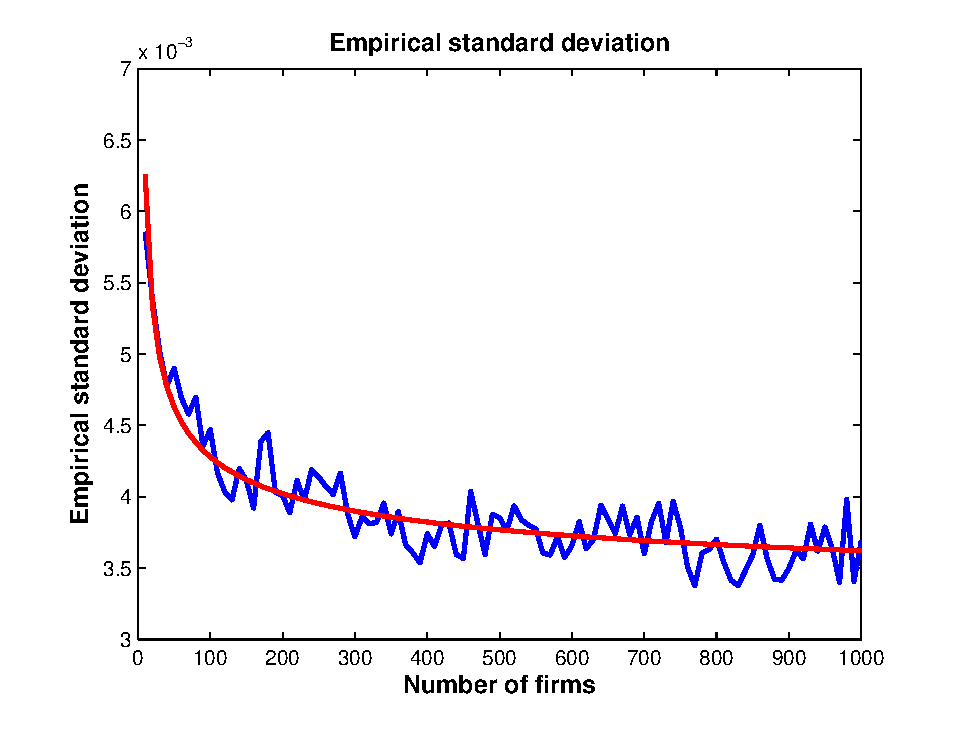
\includegraphics[scale=0.8]{simulation.eps} 
\end{center}
\caption{Empirical standard deviation as a function of $N$ (blue) and a fit to $1/\log(N)$ (red).\label{Emp_std}}
\end{figure}

\clearpage

\bibliographystyle{plain}
\bibliography{bibliotheque.bib}




\end{document}